\chapter{Fejlesztői dokumentáció} % Developer guide
\label{ch:impl}

\section{Tervezés}

\subsection{Probléma leírása}

\subsection{Felhasználói esetek}
\todo{Ez a kép nem felel meg a margónak, az baj? Legalább átlátható}
A felhasználói esetek a következőképpen néznek ki. A vállalkozó egyben felhasználó is, a felhasználók összes funkcióját tudják használni, ezt nem jelöltem a diagrammban, hogy átlátható maradjon.

\begin{figure}[H]
	\noindent\makebox[\textwidth]{
	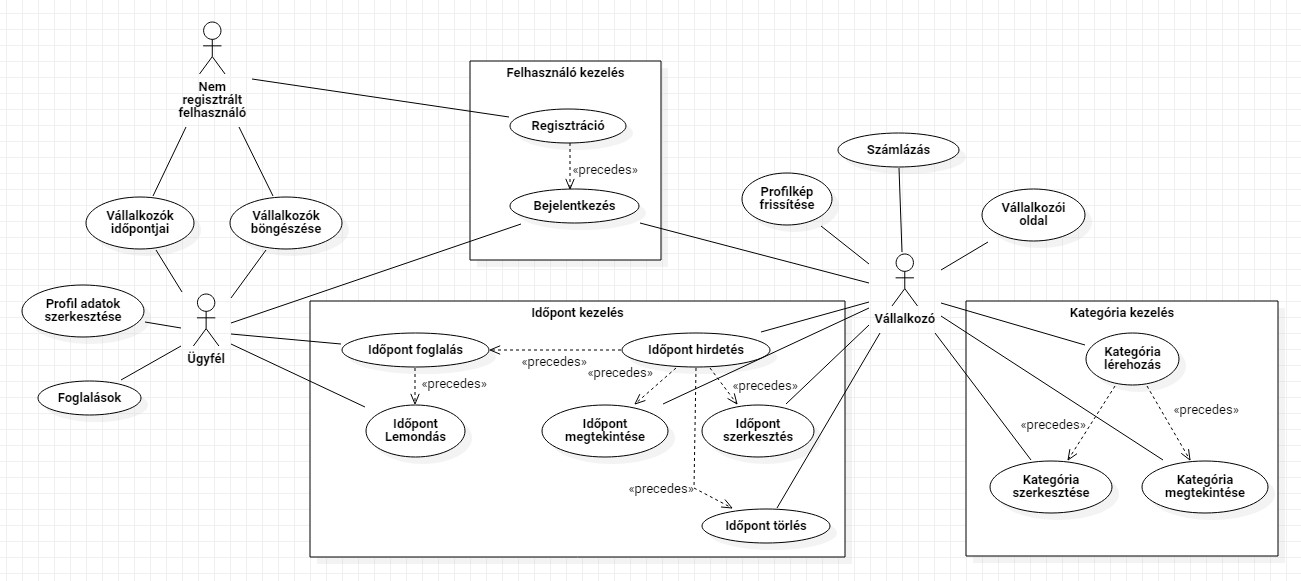
\includegraphics[width=1.3\textwidth]{usecase}}
	\caption{Felhasználói esetek}
	\label{fig:usecases}
\end{figure}

\begin{table}[H]
	\centering
	\begin{tabular}{|l|l|c|}
		\hline
		& \textbf{Leírás} & \textbf{Kód} \\
		\hline
		GIVEN & Nincs bejelentkezve & \multirow{3}{*}{asd} \\ \cline{1-2}
		WHEN & Bejelentkezéshez kötött oldalt nyitna meg & \\ \cline{1-2}
		THEN & Visszairányítódik a főoldalra & \\ 
		\hline
		GIVEN & asd & \multirow{3}{*}{asd} \\ \cline{1-2}
		WHEN & asd & \\ \cline{1-2}
		THEN & asd & \\ 
		\hline
		GIVEN & asd & \multirow{3}{*}{asd} \\ \cline{1-2}
		WHEN & asd & \\ \cline{1-2}
		THEN & asd & \\ 
		\hline
		GIVEN & asd & \multirow{3}{*}{asd} \\ \cline{1-2}
		WHEN & asd & \\ \cline{1-2}
		THEN & asd & \\ 
		\hline
		GIVEN & asd & \multirow{3}{*}{asd} \\ \cline{1-2}
		WHEN & asd & \\ \cline{1-2}
		THEN & asd & \\ 
		\hline
		GIVEN & asd & \multirow{3}{*}{asd} \\ \cline{1-2}
		WHEN & asd & \\ \cline{1-2}
		THEN & asd & \\ 
		\hline
		GIVEN & asd & \multirow{3}{*}{asd} \\ \cline{1-2}
		WHEN & asd & \\ \cline{1-2}
		THEN & asd & \\ 
		\hline
	\end{tabular}
\end{table}

\subsection{REST API vs MVC architektúra}
Webes alkalmazások körében régebben elterjedt volt a Modell-View-Controller architektúra (röviden MVC). Röviden ez azt jelenti, hogy a felhasználó akcióira a Controller réteg eldönti, hogy az állapotot (Modellt) hogy kell frissíteni, ez után pedig egy nézetet (View-t) ad vissza a felhasználónak. A gyakorlatban ez szerver oldali renderelést jelent, például a felhasználó elküld egy űrlapot a szervernek, az feldolgozza és egy szerver által renderelt HTML fájlt küld vissza a felhasználó böngészőjének.

Ennek a megközelítésnek vannak előnyei, többek között, hogy az alkalmazásnak egy kódbázisa van, egyszerűbb egy új funkciót implementálni, kevesebb technológiát is elég ismerni. Hátránya viszont, hogy dinamikus felhasználói felületet nehéz benne építeni, más alkalmazásokba, például mobil alkalmazásba, nem lehet integrálni.

Ezekre nyújt megoldást, ha a logikát egy REST API (Representational state transfer, Application Programming Interface) valósítja meg backenden, a megjelenítésért pedig egy másik program felel frontend-en. A REST egy interfész leíró struktúra, legtöbb esetben HTTP protokoll alapú kommunikációt ír le, melyben JSON formátumú adattal lehet kommunikálni.

Mivel az API-t így programatikusan tudjuk elérni, ezért más alkalmazásokkal egyszerűen képes kommunikálni. Így lehet például web-ről, telefonos- vagy asztali alkalmazásból elérni a biznisz logikát, ezért csak a megjelenítést kell variálni platformok között.

A REST API állapot mentes, ami azt jelenti, hogy a szerver nem függ valamilyen kontextustól, csak a kérésben szereplő adattal elég dolgoznia. Ez lehetővé teszi, hogy a backend több szerveren horizontálisan egy load balancer (terheléselosztó) segítségével legyen skálázva. Egy ilyen rendszerben az egymást követő kérések akár különböző backend példányokhoz futhatnak be, az alkalmazás ugyan olyan pontosan működik.

A programozható felület lehetővé teszi, hogy a szerver ne teljes oldalakat küldjön vissza válasznak, hanem csak adatot. Ez a rugalmasság lehetővé teszi, hogy a frontend dinamikus legyen. Például az én alkalmazásomban egy új időpont hirdetésénél a böngésző tesz egy kérést a szerver felé, ami visszaadja a létrejött időpont adatát és a frontend azt az egy időpontot beilleszti a jelenleg megjelenített időpontok közé, nem kell a teljes oldalt az összes időponttal újra tölteni.

A hátránya ennek az architektúrának, hogy a backend és frontend teljesen különálló, akár más programozási nyelvekben vannak írva, más eszközökkel kell fejleszteni őket, így nagyobb a projekt komplexitása. Vállalati környezetben ez előny lehet, mert külön csapatokra szét lehet osztani a frontend és backend fejlesztést. További nehézség lehet, hogy az backendet és a frontendet össze kell kötni, ez az integráció nem olyan triviális, mint egy monolitikus MVC alkalmazásban, ahol egyből a modell adatát bele lehet renderelni HTML tagek közé. Továbbá, mivel az API így egy külön álló alkalmazás, amit bárhonnan lehet lekérdezni, fontos biztonsági lépésekkel le kell védeni, hogy jogosulatlan adathoz ne lehessen hozzáférni, szennyezett adattal ne lehessen elrontani az alkalmazást.

\subsection{Clean Architecture Backenden}
\todo{Remove this paragraph}
Clean architecture, UML diagrammok, dependency injection,
repo - controller - logika interakció

Uncle Bob Clean Architecture\cite{cleanArchitecturePost}-jének a lényege, hogy az alkalmazás különböző rétegei minél kevésbé függjenek egymástól. Ő négy réteget definiál: entitások, felhasználói esetek, kontrollerek és külső szolgáltatások. Az én alkalmazásomban az entitások az alkalmazás belő reprezentációs adattagjai. A felhasználói esetek a logika osztályokban vannak, minden egyes függvény a logika osztályban egy felhasználói esetet fed le. A kontrollerek az ASP.NET-es kontrollerek. A külső szolgáltatások pedig az adatbázis kezeléssel foglalkozó repository-k és majd a jövőben az email küldő szolgáltatás.

A különböző rétegek csak egymás interfészeitől, nem implementációitól függenek. Így például a logikában nincsenek SQL lekérdezések, a kontroller nem tud fájlokat megnyitni. Ezt a függőségi befecskendezés elvével (Dependency inversion principle) valósítom meg. Ez azt jelenti, hogy egy osztály ha valami más rétegre hivatkozna, pl.: logika egy repository-ra, akkor a logika osztály konstruktora csak a repository egy interfészét várja, mert a logika szempontjából csak az a lényeg, hogy le tudjon kérdezni adatot, az nem, hogy az konkrétan hogy történik.

Ez lehetővé teszi, hogy a különböző szolgáltatásokat egyszerűen lehessen refaktorálni. Mivel minden interfészekkel dolgozik, ezért ha az adatbázis elérést Entity Framework-ről lecserélném általam írt SQL lekérdezésekre, akkor csak a repository implementációt kell megváltoztatnom és betartani az interfészt és ugyan úgy működik az alkalmazás.


Az entitásaim a következőféleképpen néznek ki:

\todo{entity uml}

Az entitások mellett DTO\footnote{Data Transfer Object - Adatátviteli objektum}-kat is használtam, a REST API ezekkel az adatszerkezetekkel kommunikál.

\todo{dto uml}

A logikát megvalósító osztályaimat entitásonként különítettem el, azaz az egy fajta entitással dolgozó felhasználói esetek tipikusan egy osztályba kerültek. A logika osztályban lehet először látni a függőségi befecskendezés elvét. A logika osztályok csak a releváns repository-k interfészeit kapják meg.

\todo{logic uml}

A kontrollerek ugyan azokat a felhasználói eseteket fedik le, mint a logika osztályok. A különbség, hogy a bejövő HTTP kéréseket kezelik, alakítják át a logikának megfelelő adatra, utána meghívják a logika egy függvényét, majd a visszakapott belső reprezentációs adatot mapp-elik DTO-vá.

\todo{Controller uml}

Az adat elérő repository interfészek a következők:

\todo{repo interface uml}

A repository megvalósítások nem térnek el sokban a megvalósított interfészektől:

\todo{repo implementation uml}

Mint látható, az entitásokon kívül az osztályok nem tartalmaznak állapot tárolásra szolgáló adattagokat. Ez a REST API állapotfüggetlensége miatt van. Így például a logika meg repository osztályok csak azért vannak osztályba szervezve, hogy ugyan azokat a befecskendezett függőségeket használják, ne kelljen minden methódusuknál paraméterként megadni őket. Ettől funkcionális érzetű a kód, viszont ez a unit tesztelésnél hasznos, amit a \ref{sec:unittests} részben tárgyalok.

A program komponensei a következő módon függnek egymástól:

\todo{big picture uml}

\subsection{Adatbázis - Entity Framework}
entity uml hivatkozások az előző részből

\subsection{Funkcionális Frontend}
React, react hooks, async result monád, reactive state changes


\section{Megvalósítás}
\subsection{Fejlesztési környezet}
Rider, vs code, visual studio, docker

dotnet, nuget

snowpack, node.js, yarn, react

???

\subsection{Fejlesztési döntések}
exceptions, dto-entity mappers

\subsection{Fejlesztés közben felmerült problémák}
EF many-to-many, ef virtual classes nullable, sqlite inmemory test parallelization


\section{DevOps}
\subsection{CI/CD}
Github actions, cd dockerrel(?)
\subsection{Docker}
Dockerfile, dockerfile optimalizáció (alpine, builder, instruction layering - caching), docker compose

\section{Tesztelés}
\subsection{Unit tesztek}
\label{sec:unittests}
Clean architecture, dependency injection, mockolás

\subsection{Integrációs tesztek}
httpclient, sqlite inmemory

\subsection{Manuális tesztek}
frontend tesztelés
























% Lorem ipsum dolor sit amet, consectetur adipiscing elit. Duis nibh leo, dapibus in elementum nec, aliquet id sem. Suspendisse potenti. Nullam sit amet consectetur nibh. Donec scelerisque varius turpis at tincidunt.


% \section{Tételek, definíciók, megjegyzések} % Theorem-like items

% \begin{definition}
% Mauris tristique sollicitudin ultrices. Etiam tristique quam sit amet metus dictum imperdiet. Nunc id lorem sed nisl pulvinar aliquet vitae quis arcu. Morbi iaculis eleifend porttitor.
% \end{definition}

% Maecenas rutrum eros sem, pharetra interdum nulla porttitor sit amet. In vitae viverra ante. Maecenas sit amet placerat orci, sed tincidunt velit. Vivamus mattis, enim vel suscipit elementum, quam odio venenatis elit, et mollis nulla nunc a risus. Praesent purus magna, tristique sed lacus sit amet, convallis malesuada magna. Phasellus faucibus varius purus, nec tristique enim porta vitae.

% \begin{theorem}
% Nulla finibus ante vel arcu tincidunt, ut consectetur ligula finibus. Mauris mollis lectus sed ipsum bibendum, ac ultrices erat dictum. Suspendisse faucibus euismod lacinia. Etiam vel odio ante.
% \end{theorem}
% \begin{proof}
% Etiam pulvinar nibh quis massa auctor congue. Pellentesque quis odio vitae sapien molestie vestibulum sit amet et quam. Pellentesque vel dui eget enim hendrerit finibus at sit amet libero. Quisque sollicitudin ultrices enim, nec porta magna imperdiet vitae. Cras condimentum nunc dui.
% \end{proof}

% Donec dapibus sodales ante, at scelerisque nunc laoreet sit amet. Mauris porttitor tincidunt neque, vel ullamcorper neque pulvinar et. Integer eu lorem euismod, faucibus lectus sed, accumsan felis. 

% \begin{remark}
% Nunc ornare mi at augue vulputate, eu venenatis magna mollis. Nunc sed posuere dui, et varius nulla. Sed mollis nibh augue, eget scelerisque eros ornare nec. Praesent porta, metus eget eleifend consequat, eros ligula eleifend ex, a pellentesque mi est vitae urna. Vivamus turpis nunc, iaculis non leo eget, mattis vulputate tellus.
% \end{remark}

% Fusce in aliquet neque, in pretium sem. Donec tincidunt tellus id lectus pretium fringilla. Nunc faucibus, erat pretium tempus tempor, tortor mi fringilla neque, ac congue ex dui vitae mauris. Donec pretium et quam a cursus.

% \begin{note}
% Aliquam vehicula luctus mi a pretium. Nulla quam neque, maximus nec velit in, aliquam mollis tortor. Aliquam erat volutpat. Curabitur vitae laoreet turpis. Integer id diam ligula.
% \end{note}

% Ut sollicitudin tempus urna et mollis. Aliquam et aliquam turpis, sed fermentum mauris. Nulla eget ex diam. Donec eget tellus pharetra, semper neque eget, rutrum diam.

% \subsection{Egyenletek, matematika} % Equations, formulas

% Duis suscipit ipsum nec urna blandit, $2 + 2 = 4$ pellentesque vehicula quam fringilla. Vivamus euismod, lectus sit amet euismod viverra, dolor metus consequat sapien, ut hendrerit nisl nulla id nisi. Nam in leo eu quam sollicitudin semper a quis velit.

% $$a^2 + b^2 = c^2$$

% Phasellus mollis, elit sed convallis feugiat, dolor quam dapibus nibh, suscipit consectetur lacus risus quis sem. Vivamus scelerisque porta odio, vitae euismod dolor accumsan ut.

% In mathematica, identitatem Euleri (equation est scriptor vti etiam notum) sit aequalitatem Equation~\ref{eq:euler}:
% \begin{equation}\label{eq:euler}
% e^{i \times \pi} + 1 = 0
% \end{equation}


% \section{Forráskódok} % Source code samples

% Nulla sodales purus id mi consequat, eu venenatis odio pharetra. Cras a arcu quam. Suspendisse augue risus, pulvinar a turpis et, commodo aliquet turpis. Nulla aliquam scelerisque mi eget pharetra. Mauris sed posuere elit, ac lobortis metus. Proin lacinia sit amet diam sed auctor. Nam viverra orci id sapien sollicitudin, a aliquam lacus suscipit. Quisque ac tincidunt leo Code~\ref{src:cpp} and \ref{src:csharp}:

% \lstset{caption={Hello World in C++}, label=src:cpp}
% \begin{lstlisting}[language={C++}]
% #include <stdio>

% int main() 
% {
% 	int c;
% 	std::cout << "Hello World!" << std::endl;

% 	std::cout << "Press any key to exit." << std::endl;
% 	std::cin >> c;
	
% 	return 0;
% }
% \end{lstlisting}

% \lstset{caption={Hello World in C\#}, label=src:csharp}
% \begin{lstlisting}[language={[Sharp]C}]
% using System;
% namespace HelloWorld
% {
% 	class Hello 
% 	{
% 		static void Main() 
% 		{
% 			Console.WriteLine("Hello World!");
			
% 			Console.WriteLine("Press any key to exit.");
% 			Console.ReadKey();
% 		}
% 	}
% }
% \end{lstlisting}

% \subsection{Algoritmusok} % Algorithms

% A general Interval Branch and Bound algorithm is shown in Algorithm~\ref{alg:ibb}. One of the following selection rules is applied in Step \ref{step:selrule}.\\
% Példa forrása: \href{https://www.inf.u-szeged.hu/actacybernetica/}{Acta Cybernetica (ez egy link)}.

% \begin{algorithm}[H]
% \caption{A general interval B\&B algorithm} 
% \label{alg:ibb} 
% \textbf{\underline{Funct}} IBB($S,f$)
% \begin{algorithmic}[1] % sorszámok megjelenítése minden n. sor előtt, most n = 1
% \STATE Set the working list ${\cal L}_W$ := $\{S\}$ and the final list ${\cal L}_Q$ := $\{\}$     
% \WHILE{( ${\cal L}_W \neq \emptyset$ )} \label{alg:igoend}
% 	\STATE  Select an interval $X$ from ${\cal L}_W$ \label{step:selrule}\COMMENT{Selection rule}  
% 	\STATE Compute $lbf(X)$ \COMMENT{Bounding rule}		  
% 	\IF[Elimination rule]{$X$ cannot be eliminated}
% 		\STATE Divide $X$ into $X^j,\ j=1,\dots, p$, subintervals   \COMMENT{Division rule}
% 		\FOR{$j=1,\ldots,p$}
% 			\IF[Termination rule]{$X^j$ satisfies the termination criterion}
% 				\STATE Store $X^j$ in ${\cal L}_W$ 
% 			\ELSE
% 				\STATE Store $X^j$ in ${\cal L}_W$ 
% 			\ENDIF
% 		\ENDFOR  
% 	\ENDIF
% \ENDWHILE
% \STATE \textbf{return} ${\cal L}_Q$
% \end{algorithmic}
% \end{algorithm}
